% Partie IV condensée (FR). Figures/table reprises ; captions et en-têtes traduits,
% virgules décimales.

\noindent Nous déterminons d'abord quels textes publics fournissent un signal d'entraînement
pertinent. Nous constituons et publions des corpus biomédicaux français à partir de
sources publiques : \emph{biomed-fr}, 413 millions de mots, puis \emph{MC-Bio}, dix
milliards de tokens. Comme leurs documents mêlent contenu médical pertinent et contenu
générique, nous les annotons au niveau du paragraphe par type de contenu et par
qualité.

\begin{figure}[ht]
\centering
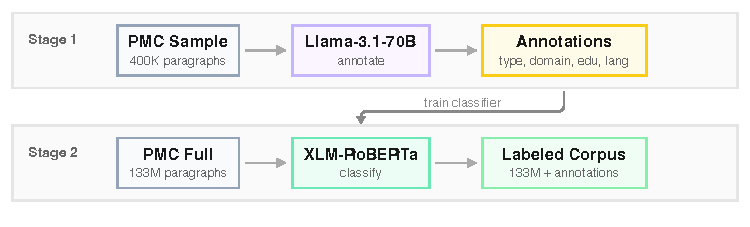
\includegraphics[width=\columnwidth]{sources/part_1/chapter2/imgs/pipeline.pdf}
\caption{\textbf{Chaîne d'annotation en deux étapes.} Étape~1 : Llama-3.1-70B annote 0,33\% des paragraphes de PMC selon quatre dimensions. Étape~2 : un XLM-RoBERTa affiné distille ces annotations pour étiqueter le corpus entier, ce qui autorise des stratégies de filtrage flexibles.}
\label{fig:pipeline}
\end{figure}

Comme le montre la \Cref{fig:pipeline}, un grand modèle annote une petite fraction de
PubMed Central selon quatre dimensions, et un encodeur affiné distille ces étiquettes
au corpus entier, ce qui rend possible un filtrage au niveau du paragraphe.
Sélectionner les paragraphes pertinents égale le pré-entraînement sur le corpus
complet avec un tiers des tokens, et sa recette clinique atteint le même point avec
2,5 fois moins de tokens. Le filtre a aussi fait remonter environ deux millions de cas
cliniques présents à l'intérieur d'articles scientifiques, décrits au passage et
jamais étiquetés comme texte clinique, que nous avons publiés comme un ensemble ouvert
de cas cliniques.

La qualité n'est pas uniforme dans le corpus : les revues et les études obtiennent les
scores de valeur éducative les plus élevés, le texte clinique varie davantage, et le
contenu générique en obtient rarement, ce qui rend le filtrage au niveau du paragraphe
utile.

Quels signaux de qualité aident réellement est moins évident qu'il n'y paraît. Nous
annotons chaque passage selon quatre signaux — valeur éducative, richesse du contenu,
qualité de rédaction et précision terminologique — sur les 2,16 millions de passages
annotés. En les retirant un à un, nous constatons que la valeur éducative et la
richesse du contenu améliorent les performances, tandis que la qualité de rédaction et
la précision terminologique les dégradent. Nous montrons aussi que les filtres
neuronaux de qualité génériques peuvent amplifier la contamination des jeux
d'évaluation : un filtre réglé pour le web généraliste ne peut donc être utilisé sur
du texte biomédical sans vérifier ce qu'il sélectionne.
